\documentclass[pdftex,12pt,a4paper]{article}
%\documentclass{report}
\usepackage{amsmath}
\usepackage{fullpage}
\usepackage{pdfpages}
\usepackage{listings}
\usepackage{longtable}
\usepackage{verbatim}
\newcommand{\HRule}{\rule{\linewidth}{0.5mm}}
\newcommand{\nspace}{\\[0.25cm]}
\newcommand{\lspace}{\\[0.50cm]}
\newcommand{\Lspace}{\\[1.0cm]}


\title{Design and Analysis of Algorithms Course Project}
\author{Jonathan Gillett \& Joseph Heron \& Amit Jain}



\begin{document}
\pagestyle{empty}
\begin{titlepage}
  		\newlength{\saveparindent}
		\setlength{\saveparindent}{\parindent}
		\setlength{\parindent}{0cm}
  		\sf
		\center
 
  		\HRule\\[0.60cm]
			\textsc{\Huge Design and Analysis of Algorithms}\\[0.25cm] 
			\textsc{\Huge Course Project}\\[0.50cm]
		\HRule\\[5cm]
		\textsc{\LARGE Jonathan Gillett \qquad Joseph Heron}\\[0.65cm]
		\textsc{\LARGE Amit Jain}\\[6.5cm]
		\textsc{\LARGE{}\today}\\

  		\setlength{\parindent}{\saveparindent}
\end{titlepage}


% Flush everything to the left
\flushleft


\textsc{\Huge Convex Hull Algorithm} \hfill \Lspace


% Description of convex hull algorithms (take from wikipedia
\textsc{\Large Description} \hfill \nspace

The convex hull is the set of points such that they form the smallest convex hull that encompasses the set of all points within the hull. A typical analogy for the convex hull is that it can be thought of as a set of points, such that when a rubber band is stretched around them it forms the
convex hull of a set of points.

\begin{figure}[h!]
  \centering
	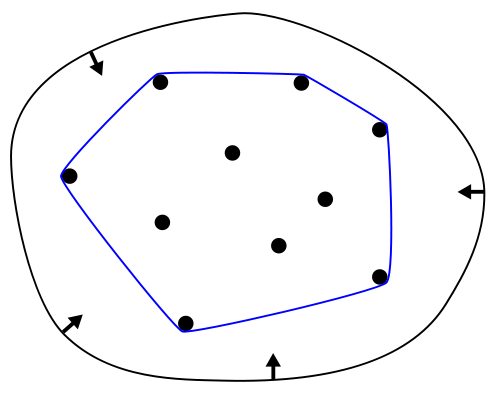
\includegraphics[scale=0.4]{img/convexhull_rubberband.png}
	\caption{http://commons.wikimedia.org/wiki/Image:ConvexHull.png}
\end{figure}

The convex hull algorithms are used to determine the convex hull of a finite set of points,
currently there are several well-known algorithms used to determine the convex hull of a finite
set of points such as: Jarvis March, Graham Scan, QuickHull, Monotone Chain, Marriage-Before-Conquest, and Chan's Algorithm.  Currently the best algorithmic complexity for the convex hull algorithm is $O(n log h)$, which Chan's algorithm being the most recently published optimal  convex hull algorithm.\nspace

% ADD CITATION FOR BIG-O COMPLEXITY, CHAN'S ALGORITHM

For our project we decided to use the Monotone Chain algorithm, which as a worst-case complexity
of $O(n log n)$, while it is not as optimal as Chan's algorithm or Marriage-Before-Conquest the Monotone Chain algorithm is better understood and more widely used due to the ease of impementation.\lspace

% Citation

% Description of algorithm, explanation of the code
\textsc{\Large Monotone Chain Algorithm} \hfill \nspace


% Sample Results
\textsc{\Large Sample Results} \hfill \nspace

\textsc{\large Sample Result 1} \hfill \nspace

\textsc{\large Sample Result 2} \hfill \nspace

\textsc{\large Sample Result 3} \hfill \nspace

\textsc{\large Sample Result 4} \hfill \nspace


% Complexity Analysis
\textsc{\Large Complexity Analysis} \hfill \nspace


% Conclusion
\textsc{\Large Concluding Remarks} \hfill \nspace



\begin{thebibliography}{9}

\bibitem{lamport94}
  Leslie Lamport,
  \emph{\LaTeX: A Document Preparation System}.
  Addison Wesley, Massachusetts,
  2nd Edition,
  1994.

\end{thebibliography}

\end{document}
